\documentclass[a4paper]{report}
\usepackage{fullpage}
\usepackage{color}
\usepackage{caption}
\usepackage{tocloft}
\usepackage{float}
\usepackage[utf8]{inputenc}
\usepackage[T1]{fontenc}
\usepackage[french]{babel}
\usepackage{graphicx}
\usepackage{titlesec}
\usepackage{listings}
\usepackage{beraserif}
\usepackage{hyperref}
\usepackage{xcolor}
\lstset{language=Java,
basicstyle=\small\ttfamily,
keywordstyle=\color{blue},
        commentstyle=\color{green},
        stringstyle=\color{red},
        showstringspaces=false,
        breaklines=true,
        xleftmargin=-8mm}


\definecolor{navyblue}{RGB}{39,66,94}

\titleformat{\chapter}[display]
    {\bfseries\huge\color{navyblue}}{\chaptertitlename\ \thechapter}{18pt}{}
          
\titleformat{\section}
    {\bfseries\Large\color{navyblue}}{\thesection}{1em}{}
        
\titleformat{\subsection}
    {\color{navyblue}\normalfont\large}
    {\color{navyblue}\thesubsection}{1em}{}

\begin{document}

\begin{titlepage}
    \centering
    
    
\includegraphics[width=0.3\textwidth]{logo/logo_univ_bordeaux.png}\par\vspace{1cm}
    
    {\scshape\LARGE Université de Bordeaux\par}
    \vspace{1cm}
    {\scshape\Large Master 1 Génie Logiciel\par}
    \vspace{3cm}
    {\Large\bfseries Rapport de Projet de Programmation:\par}
    \vspace{1cm}
    {\Huge {Conception d'une application web pour la gestion d'un cabinet médical}\par}

    \vspace{2.5cm}
    \noindent\rule{0.6\textwidth}{0.7pt}
    \vspace{0.5cm}

    \vspace{4cm}
    \begin{tabular}{@{}p{0.5\linewidth}p{0.5\linewidth}@{}}
    \raggedright
    {\large\itshape Réalisé par\par}
    \vspace{0.5cm}
    {\Large Ephrem Jennifer\\Loustau Valentin\\Duboureau Guillaume\\Goudoussy Diallo Abdoul\par}
    &
    \vspace{1cm}
    \raggedleft
    {\large\itshape Encadré par\par}
    {\Large Mme Sarah Fara Ouada\par}
    \vspace{0.5cm}

    {\large Année universitaire 2022-2023\par}
    \end{tabular}
    
\end{titlepage}
\let\cleardoublepage\clearpage
\tableofcontents
\newpage
\listoffigures


\chapter{Introduction}

La gestion d'un cabinet médical peut vite devenir compliquée pour les professionnels de santé. L'analyse, la collecte et la gestion des données sont des éléments 
clés pour fournir des soins de qualité aux patients. Pour faciliter ces tâches, nous avons conçu une application de gestion d'un cabinet 
médical qui permettra aux professionnels de santé de gérer efficacement leurs rendez-vous, les dossiers médicaux ainsi que les ordonnances de leurs patients. 
Notre interface intuitive et simple d'utilisation permettra aux patients de trouver un rendez-vous avec le spécialiste de leur choix en un rien de temps. \newline\newline
L'objectif et la problématique, ici, est de concevoir une application web qui soit la mieux construite possible. Cela permettra ainsi d'avoir une gestion d'un cabinet 
médicale la plus simple et fluide possible. Pour cela, nous devrons répondre à certains besoins, que nous détaillerons dans les parties suivantes, tels que la centralisation des dossiers médicaux
et de facilité la navigation et l'expérience utilisateur, que se soit pour le médecin ou la patient.
 \newline\newline
Dans ce rapport, nous allons décrire en détail la conception de cette application en expliquant les choix que nous avons faits 
pour les différentes fonctionnalités. Nous fournirons un cahier d'analyse des besoins avec des diagrammes de cas d'utilisations et
un diagramme de classe pour illustrer la conception de l'application. Nous présenterons également 
les technologies et outils que nous avons utilisés pour développer cette application, notamment ReactJS et Java.
Vous trouverez en dernière partie de ce rapport, toutes les fonctionnalités, imagées, que nous avons implémentées.
\newline\newline
Enfin, nous discuterons des améliorations futures possibles de notre application et des opportunités d'extension de ses fonctionnalités.

\chapter{Analyse des besoins}\label{besoins}
\section{Identification des acteurs}

Un acteur représente un rôle joué par une personne externe ou par un processus qui interagit avec le système.
\newline\newline
Les acteurs de notre système sont :
\newline
\begin{itemize}
    \item[$\bullet$] \textbf{Patient} : il s’agit d’un acteur qui utilise le site pour gérer 
    (ajouter, consulter, supprimer) ses rendez-vous, consulter son dossier médical. 
    Il peut également mettre à jour ses informations personnelles et communiquer ses infos au médecin.
    \item[$\bullet$] \textbf{Médecin} : il s’agit d’un acteur qui gère les dossiers des patients, prescrit des ordonnances et 
    les imprime. Il s’occupe de la gestion des rendez-vous de ses patients et les notifie s’il effectue 
    quelconque modification.
  \end{itemize}
  
\section{Les besoins fonctionnels}
\subsection{Pour le patient}
\begin{enumerate}
    \item Création de compte\newline
        \begin{itemize}
            \item[$\bullet$] \underline{Quantifications}: Pouvoir créer qu’un seul compte par adresse mail.
            \item[$\bullet$] \underline{Contraintes ou difficultés techniques}: Sécurité des données personnelles des patients.
            \item[$\bullet$] \underline{Énonciation des risques et parades}: Risque de vols des données.\newline
            \textbf{Parade}: Protocole de sécurité pour protéger les données.
            \item[$\bullet$] \underline{Spécification des tests de contrôle}: Tests unitaires.\newline
        \end{itemize}

    \item Gestion et consultation des rendez-vous en ligne\newline
    \begin{itemize}
        \item[$\bullet$] \underline{Quantifications}: Pouvoir prendre plusieurs rendez-vous selon les créneaux libres sur le planning. 
        De plus, possibilité de visualiser ses rendez-vous en temps réel.
        \item[$\bullet$] \underline{Éléments de faisabilité}: Mettre en place un système de gestion de rendez-vous en ligne tel que doctolib et vérifier sa faisabilité.
        \item[$\bullet$] \underline{Contraintes ou difficultés techniques}: Assurer la synchronisation en temps réel avec le calendrier du médecin, garantir la disponibilité d’un rendez-vous.
        \item[$\bullet$] \underline{Énonciation des risques et parades}: Chevauchement de prise de rendez-vous pour des patients différents, ou sélectionner un rendez-vous qui n'existe plus.\newline
        \textbf{Parade}: Bloquer la prise d’un rendez-vous pour le premier arrivé.
        \item[$\bullet$] \underline{Spécification des tests de contrôle}: Tests unitaires.
    \end{itemize}
        
\end{enumerate}

\subsection{Pour le médecin}

\begin{enumerate}
    \item Gérer (ajouter/modifier/supprimer documents) les dossiers médicaux des patients \newline
    \begin{itemize}
        \item[$\bullet$] \underline{Quantifications}: Vue complète des dossiers des patients en temps réel.
        \item[$\bullet$] \underline{Éléments de faisabilité}: Évaluation de différents systèmes de dossiers médicaux pour comprendre les fonctionnalités.
        \item[$\bullet$] \underline{Contraintes ou difficultés techniques}: Sécurité des données.
        \item[$\bullet$] \underline{Énonciation des risques et parades}: Risques de pertes de données à cause d’un souci technique, risque de non synchronisation/mise à jour.\newline
        \textbf{Parade}: Historique de sauvegarde.
        \item[$\bullet$] \underline{Spécification des tests de contrôle}: Tests de sécurité.\newline
    \end{itemize}

    \item Gestion de ses rendez-vous en ligne\newline
    \begin{itemize}
        \item[$\bullet$] \underline{Quantification}: Possibilité de visualiser son calendrier de rendez-vous en temps réel.
        \item[$\bullet$] \underline{Éléments de faisabilité}: Mettre en place un système de gestion de rendez-vous en ligne tel que doctolib et vérifier sa faisabilité.
        \item[$\bullet$] \underline{Contraintes ou difficultés techniques}: Assurer la synchronisation en temps réel avec le calendrier, garantir la disponibilité d’un rendez-vous 
        (ne pas placer le rendez-vous sur le créneau d’un autre patient, dû à une synchronisation non effectué).
        \item[$\bullet$] \underline{Énonciation des risques et parades}: Rendez-vous en simultané pour des patients différents, sélectionner un rendez-vous qui n'existe plus.\newline
        \textbf{Parade}:  Bloquer la prise d’un rendez-vous pour le premier arrivé.
        \item[$\bullet$] \underline{Spécification des tests de contrôle}: Tests unitaires. \newline
    \end{itemize}

    \item Communication avec les patients\newline
    \begin{itemize}
        \item[$\bullet$] \underline{Éléments de faisabilité}: Mise en place d’un système de notifications par e-mail. 
        \item[$\bullet$] \underline{Contraintes ou difficultés techniques}: Aucune contrainte. \newline
    \end{itemize}

    \item Consulter son planning des rendez-vous\newline
    \begin{itemize}
        \item[$\bullet$] \underline{Quantification}: Le médecin doit pouvoir consulter son planning pour chaque jour de la semaine, ainsi que pour une période donnée : 1 semaine.
		Le planning doit être mis à jour en temps réel lorsque des rendez-vous sont ajoutés ou supprimés.
        \item[$\bullet$] \underline{Éléments de faisabilité}: La consultation du planning peut être réalisée en utilisant une interface graphique simple, qui affiche les rendez-vous (stockés dans une base de données) 
        en fonction de l'heure et de la date tel que le logiciel Google Calendar.
        \item[$\bullet$] \underline{Contraintes ou difficultés techniques}: Garantir la confidentialité des informations stockées dans la base de données.
        \item[$\bullet$] \underline{Énonciation des risques et parades}:  Risque que les rendez-vous soient compromis si la base de données est piratée. Risque que le planning du médecin ne soit pas à jour après modification.\newline
        \textbf{Parade}: Le système peut être conçu pour utiliser des méthodes de cryptage pour protéger les données sensibles. Actualisation du planning après chaque modification.
        \item[$\bullet$] \underline{Spécification des tests de contrôle}: Des tests de validation peuvent être effectués pour vérifier que le système affiche correctement les rendez-vous dans l'interface utilisateur. Des tests de contrôle 
        peuvent être effectués pour vérifier que les données sont correctement stockées dans la base de données et affichées dans l'interface utilisateur.\newline
    \end{itemize} 

    \item Bilan de santé (Le système doit assurer l’impression des fiches malades et les bilans): \newline
    \begin{itemize}
        \item[$\bullet$] \underline{Contraintes ou difficultés techniques}: Les fichiers doivent être au format PDF exclusivement pour ne pas perdre d’informations et pour une meilleure impression.
        \item[$\bullet$] \underline{Énonciation des risques et parades}: Risque de mauvais transfert/perte de données lors de l’envoie du bilan par le médecin au patient.\newline
        \textbf{Parade}: Nous pourrons vérifier si le document reçu par le patient est vide (null) ou non.
    \end{itemize}
\end{enumerate}

\section{Les besoins non-fonctionnels}

Ce sont des besoins en relation avec la performance du système, la facilité d’utilisation,
l’ergonomie des interfaces, la sécurité etc. Et parmi ces besoins nous citons :
\begin{enumerate}
    \item Sécurité des données médicales des patients\newline
    \begin{itemize}
        \item[$\bullet$] \underline{Éléments de faisabilité}: Mise en place d’un système d’identification et d’authentification de chaque utilisateur (patients/médecins) pour garantir que seuls les utilisateurs autorisés aient accès au système et aux données sensibles.
        \item[$\bullet$] \underline{Contraintes ou difficultés techniques}: Complexité de la gestion des autorisations d'accès pour les différents utilisateurs.
        \item[$\bullet$] \underline{Énonciation des risques et parades}: Risque de faille et accès à un intrus aux données des patients.\newline
        \textbf{Parade}: Il faudrait pour cela protéger ces données.
        \item[$\bullet$] \underline{Spécification des tests de contrôle}: Connexion au logiciel avec les différents acteurs et vérifier leur autorisation (un patient n’a pas accès au rendez-vous de tous les patients par exemple). \newline
    \end{itemize}

\item Simplicité et ergonomie de l’interface graphique\newline
\begin{itemize}
    \item[$\bullet$] \underline{Éléments de faisabilité}: Mise en place d’une interface intuitive et facile à utiliser pour les utilisateurs, 
    en utilisant des icônes, des boutons et d'autres éléments de conception familiers (système de navigation logique), avec des choix judicieux de couleurs, 
    de polices et d’images pour renforcer la clarté et la lisibilité de l'interface.
    \item[$\bullet$] \underline{Contraintes ou difficultés techniques}: Temps nécessaire pour trouver le juste équilibre entre simplicité et fonctionnalité 
    mais aussi pour la conception et la mise en œuvre d’une telle interface.
    \item[$\bullet$] \underline{Énonciation des risques et parades}: Risque de confusion pour les utilisateurs et bug de navigation.\newline
    \textbf{Parade}: Il faudrait faire tester le logiciel par plusieurs utilisateurs et recueillir un feedback.
    \item[$\bullet$] \underline{Spécification des tests de contrôle}: Tests unitaires.	\newline
\end{itemize}

\item Performance du système en temps de réponse, stockage mémoire

\begin{itemize}
    \item[$\bullet$] \underline{Quantification}: Temps de réponses en fonction des différentes actions (pour une requête utilisateur, pour le chargement d'une page).
    \item[$\bullet$] \underline{Éléments de faisabilité}: Un essai peut être implémenté pour mesurer la performance actuelle du système et trouver des améliorations à faire.
    \item[$\bullet$] \underline{Contraintes ou difficultés techniques}: Posséder un stockage suffisant pour contenir toutes les données enregistrées, réussir à élaborer des algorithmes pour exécuter les requêtes en temps réel.
    \item[$\bullet$] \underline{Énonciation des risques et parades}:  Les risques peuvent être un stockage insuffisant en mémoire.\newline
    \textbf{Parade}: Utilisation de technologies de stockage plus performantes.
    \item[$\bullet$] \underline{Spécification des tests de contrôle}: Tests de performance pour mesurer les temps de réponse, tests de stockage pour vérifier que la mémoire est suffisante.
\end{itemize} 

\end{enumerate}

\section{Diagrammes de cas d'utilisation}

\subsection{Créer un compte}
\begin{figure}[H]
    \vspace{-10pt}
    \centering
    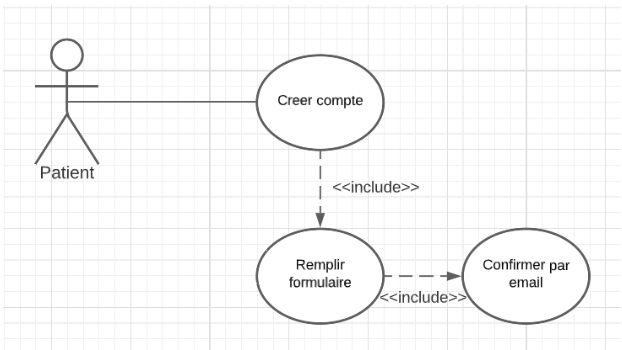
\includegraphics[width=0.5\textwidth]{besoins/creer-compte.png}
    \caption{Diagramme de cas d'utilisation : créer un compte}
    \label{fig:DCU1}
\end{figure}

\subsection{S'authentifier}
\begin{figure}[H]
    \vspace{-10pt}
    \centering
    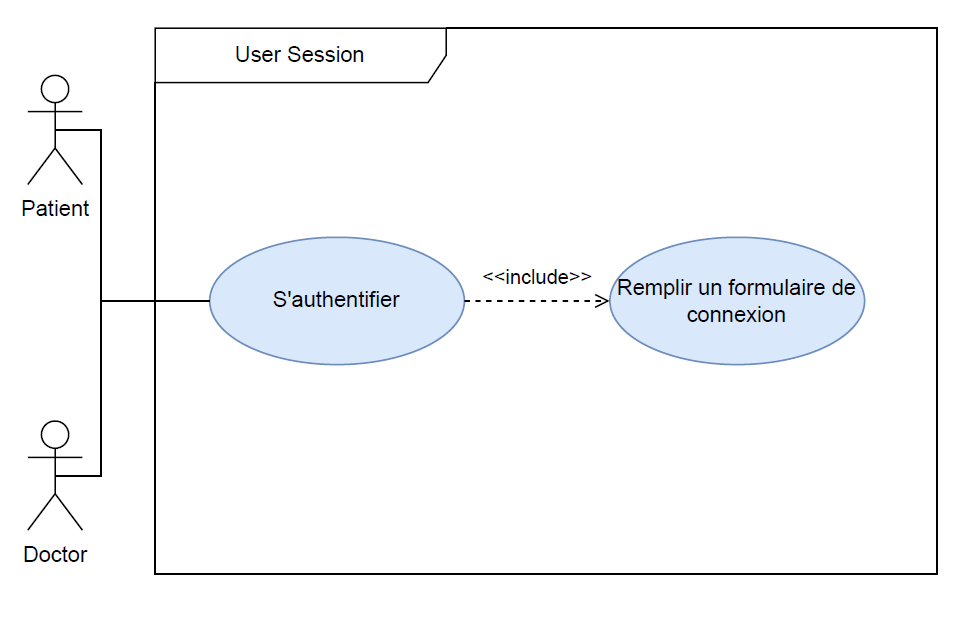
\includegraphics[width=0.5\textwidth]{besoins/authentification.png}
    \caption{Diagramme de cas d'utilisation : s'authentifier}
    \label{fig:DCU2}
\end{figure}

\subsection{Gérer les rendez-vous en ligne (Patient)}
\begin{figure}[H]
    \vspace{-10pt}
    \centering
    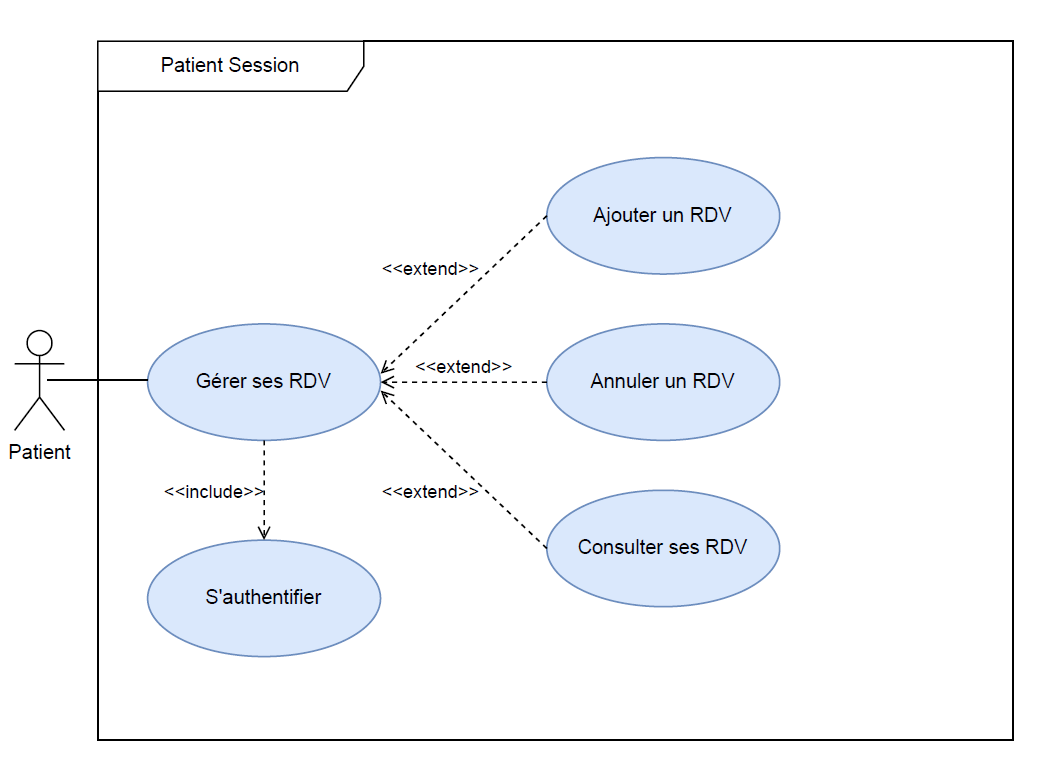
\includegraphics[width=0.5\textwidth]{besoins/gerer-rdv-patient.png}
    \caption{Diagramme de cas d'utilisation : Gérer les rendez-vous en ligne (Patient)}
    \label{fig:DCU3}
\end{figure}

\subsection{Gérer les rendez-vous en ligne (Médecin)}
\begin{figure}[H]
    \vspace{-10pt}
    \centering
    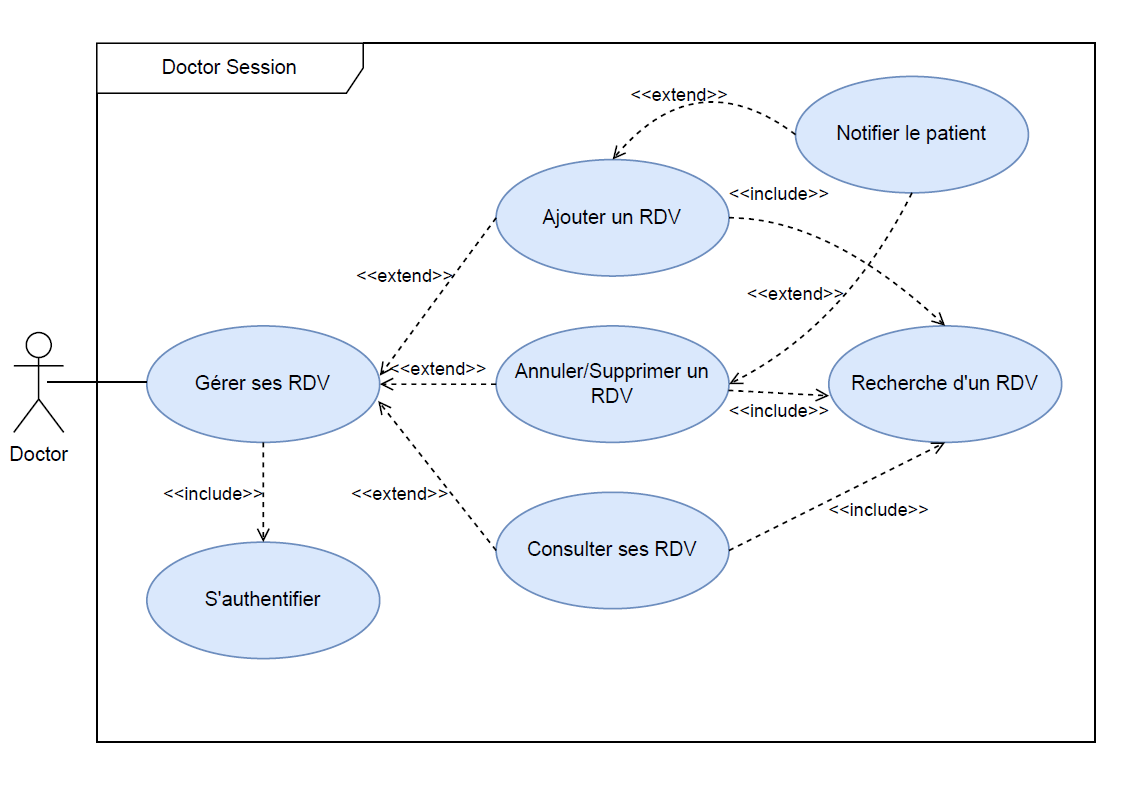
\includegraphics[width=0.5\textwidth]{besoins/gerer-rdv-medecin.png}
    \caption{Diagramme de cas d'utilisation : Gérer les rendez-vous en ligne (Médecin)}
    \label{fig:DCU4}
\end{figure}

\subsection{Consulter les rendez-vous}
\begin{figure}[H]
    \vspace{-10pt}
    \centering
    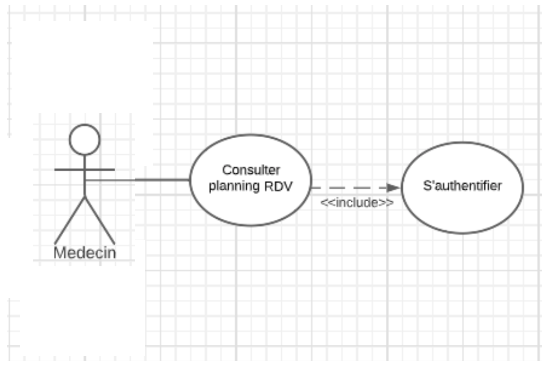
\includegraphics[width=0.55\textwidth]{besoins/consulter-rdv.png}
    \caption{Diagramme de cas d'utilisation : Consulter les rendez-vous}
    \label{fig:DCU5}
\end{figure}

\subsection{Consulter le dossier médical}
\begin{figure}[H]
    \vspace{-10pt}
    \centering
    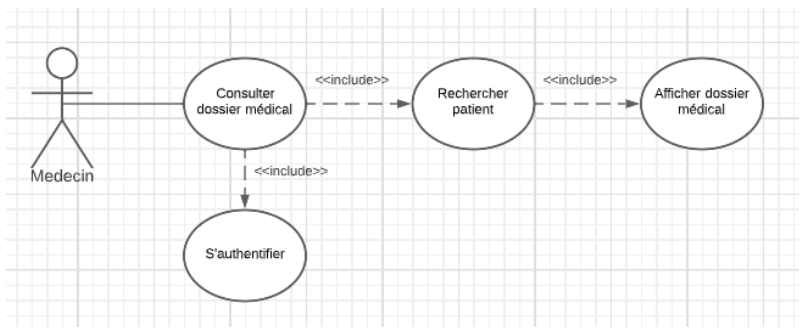
\includegraphics[width=0.6\textwidth]{besoins/consulter-dossier-medical.png}
    \caption{Diagramme de cas d'utilisation : Consulter le dossier médical}
    \label{fig:DCU6}
\end{figure}

\subsection{Gérer le dossier médical}
\begin{figure}[H]
    \vspace{-10pt}
    \centering
    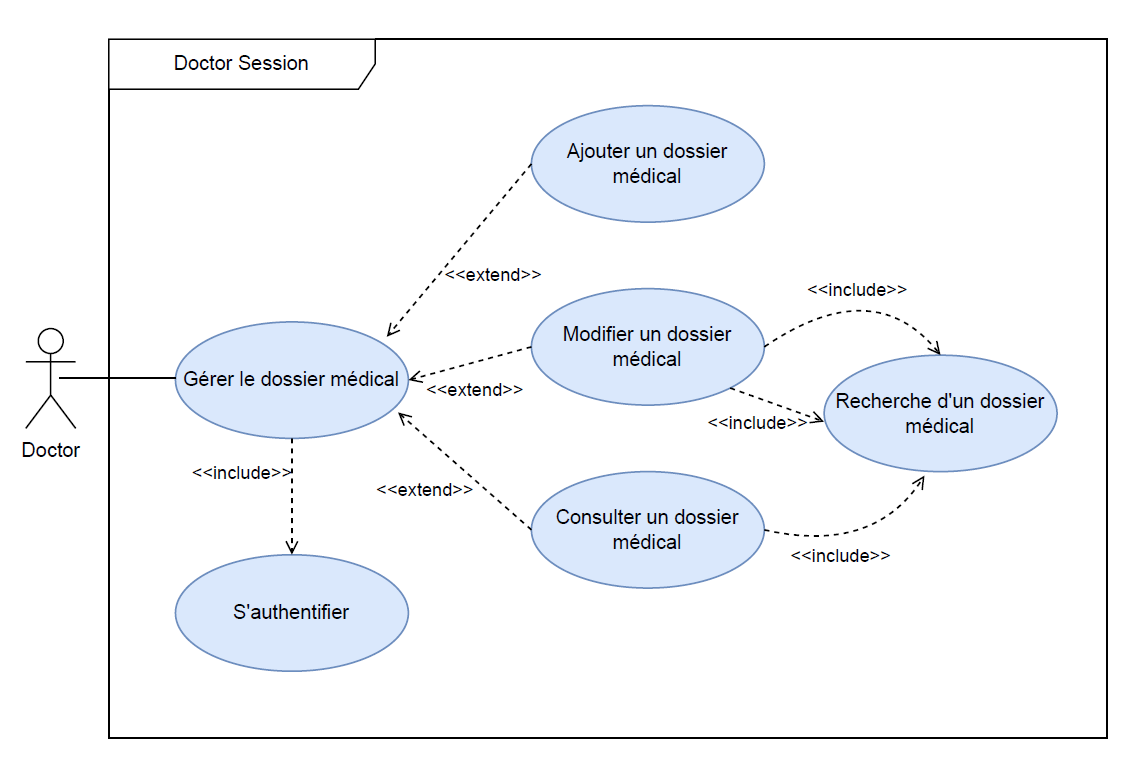
\includegraphics[width=0.5\textwidth]{besoins/gerer-dossier-medical.png}
    \caption{Diagramme de cas d'utilisation : Gérer le dossier médical}
    \label{fig:DCU7}
\end{figure}

\subsection{Génerer le bilan de santé}
\begin{figure}[H]
    \vspace{-10pt}
    \centering
    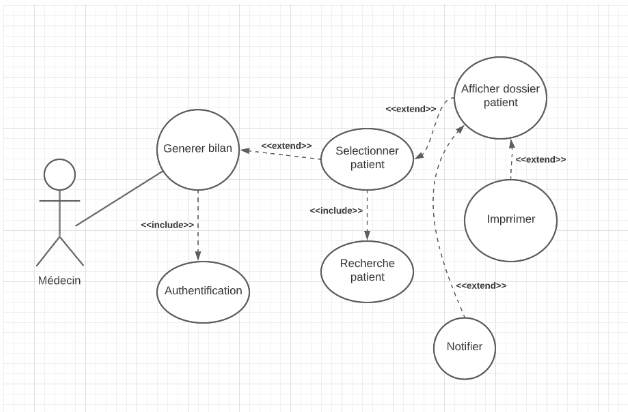
\includegraphics[width=0.5\textwidth]{besoins/bilan-sante.png}
    \caption{Diagramme de cas d'utilisation : Génerer le bilan de santé}
    \label{fig:DCU8}
\end{figure}

\section{Diagrammes de classe du Domain}
Concernant le diagramme de classe, nous avons représenté seulement les classes du Domain car elle représente le coeur de l'architecture DDD.
\begin{figure}[H]
    \vspace{-10pt}
    \centering
    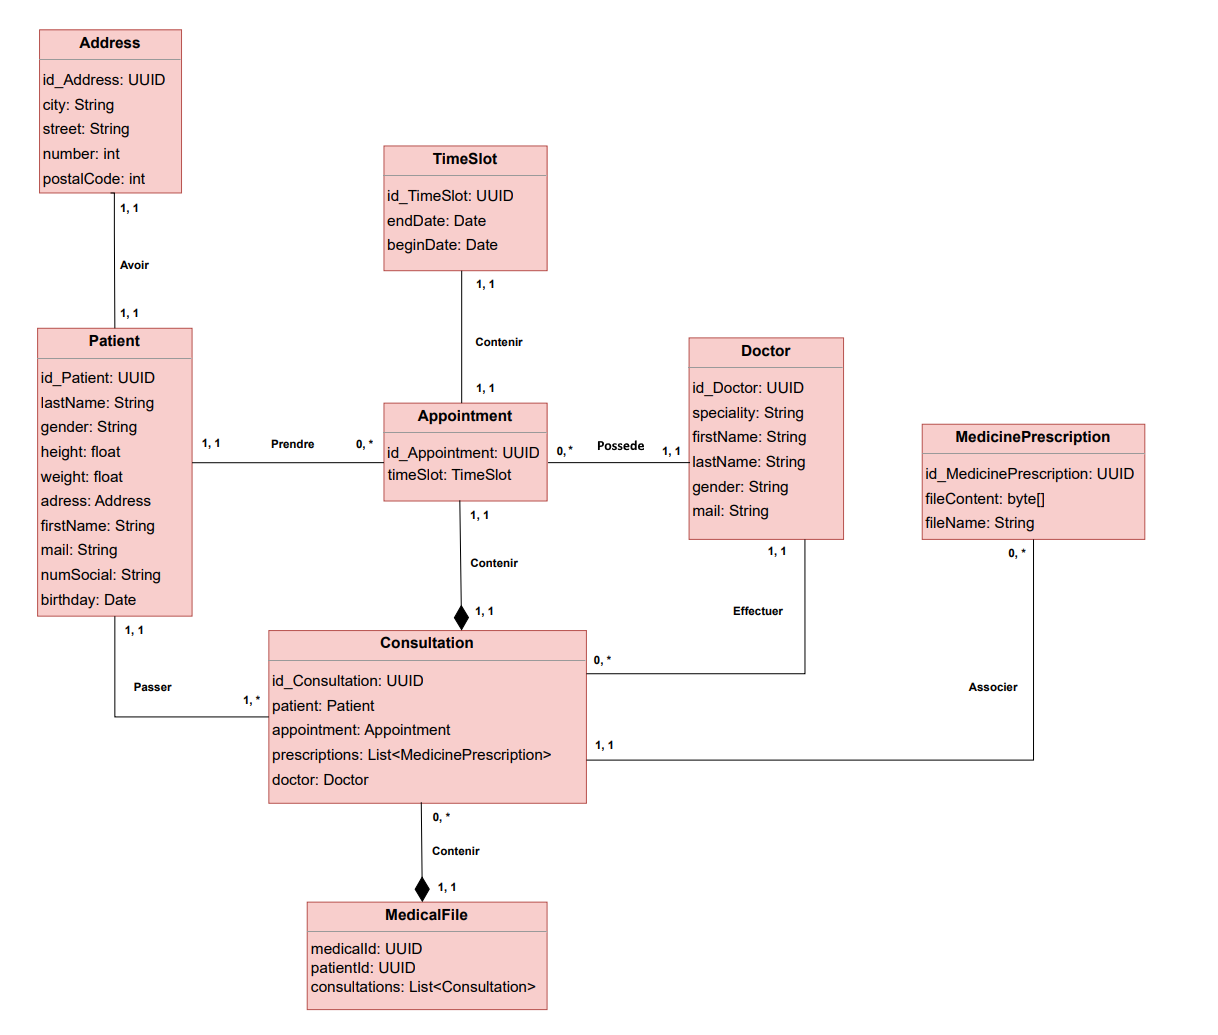
\includegraphics[width=0.85\textwidth]{besoins/class_diagram.png}
    \caption{Diagramme de classes}
    \label{fig:DCU9}
\end{figure}

\chapter{Conception}


L'architecture logicielle de notre application web pour la gestion d'un cabinet médical se compose d'un front-end, d'un back-end et d'une base de données.
Pour le back-end, nous avons décidé d'utiliser une architecture DDD (Domain-Driven Design) qui se compose de quatre couches distinctes: une couche domaine, 
une couche infrastructure, une couche application et une couche interface utilisateur. \newline \newline
Dans la couche domaine, on trouve les éléments clés de notre application tels que les patients, les médecins, les rendez-vous, les créneaux horaires, les consultations, 
les adresses des patients et les prescriptions médicales. 
Nous avons distingué les "values object" des Entity et de notre Aggrégat, le dossier médical. Ainsi, nous pouvons recréer nos objets en les récupérant de la base de données ou
alors sauvegarder ces objets. C'est ce qui nous permet de faire le pont entre la base de données et le frontend qui reçoit et met en forme les données.\newline \newline
Nous avons également mis en place une couche infrastructure en utilisant des bases de 
données relationnelles pour stocker les informations de l'application. Cette couche infrastructure est responsable de créer 
pour chaque classe du domaine une table et de gérer les requêtes et les mises à jour dans celles-ci. \newline \newline
Dans la couche interface utilisateur, on a des controllers qui servent d'intérmédiaires entre la partie client et la partie serveur. 
Les controllers reçoivent les entrées utilisateurs, les envoient à la couche application et envoient une réponse au client. Les controllers renvoient en général
une réponse HTTP afin de distinguer les différents code HTTP que l'on reçoit (ok, forbiden...) \newline \newline
Avec cette architecture DDD, nous avons créé une application structurée pour répondre aux besoins spécifiques d'un cabinet médical. Le code est ainsi plus facile à lire
car les données sont structurées par couches.\newline\newline
Concernant le frontend, nous nous occupons ici de présenter les données, et c'est donc une partie de conception graphique et de présentation aux utilisateurs et non pas une partie
de conception d'un modèle pour la modélisation du cabinet médical. Les données sont donc traitées dans le backend pour pouvoir être stockées dans la base de données.

\chapter{Réalisation}

\section{Outils de développement}

\begin{itemize}
    \item[$\bullet$] \underline{Java} : Nous avons utilisé le langage de programmation orienté objet Java pour notre projet.\newline
    \item[$\bullet$] \underline{ReactJS} : Pour le côté Front-end, nous avons utilisé la bibliothèque JavaScript ReactJS qui est très populaire dans le monde du développement web et 
    très facile d'utilisation. Elle fonctionne avec des composants où chaque composant représente une partie de l'interface utilisateur. Ces composants sont réutilisables ce qui nous permet de gagner du temps. 
    Elle possède également une documentation bien organisée et facile à comprendre. \newline
    \item[$\bullet$] \underline{Maven} : Pour la construction du projet nous avons choisi Maven, un outil de gestion de projet facile à configurer et à utiliser. Il peut être étendu grâce à des plugins pour répondre à des besoins spécifiques. \newline
    \item[$\bullet$] \underline{Git} : Pour pouvoir au mieux travailler sur ce projet chacun de notre côté, nous avons décidé d'utiliser Git qui est un logiciel de gestion de versions décentralisé. Il permet de travailler
    sur des parties différentes du code en même temps et il est très utile pour le travail en équipe.  \newline
    \item[$\bullet$] \underline{Postgresql} : Pour la gestion de notre base de données nous avons utilisé Postgresql qui est un système de gestion de bases de données relationnelles. Il est fiable et robuste, de plus 
    nous avions déjà utilisé ce système donc c'était facile pour nous de l'utiliser pour notre projet. \newline
    \item[$\bullet$] \underline{JUnit} : Pour les tests, nous avons utilisé JUnit qui est un framework de test unitaire pour Java et qui permet de tester des fragments de code de manière isolée et automatisée.\newline
\end{itemize}

\section{Côté back-end}

Pour la partie back-end, nous avons entamé le processus par l'implémentation de la couche domaine en y incluant les protagonistes majeurs 
du cabinet médical : les docteurs et les patients. Nous avons poursuivi notre travail en créant des value objects et des 
entités tels que les adresses postales, les rendez-vous, les consultations, les ordonnances et les utilisateurs. Nous avons conclu en créant l'agrégat, qui est un dossier médical. \newline\newline
Ensuite, nous avons développé la couche infrastructure en créant quatre dépôts distincts : un pour les médecins, un pour les 
patients, un pour les utilisateurs et un pour le cabinet médical dans son ensemble. Ces dépôts contiennent les requêtes et les 
insertions dans les tables de la base de données.\newline\newline
Par la suite, nous avons travaillé sur la couche application, qui récupère les informations de la couche infrastructure afin de les transmettre à la couche interface utilisateur. \newline\newline
Enfin, nous avons implémenté la couche interface utilisateur, dans laquelle se trouvent des contrôleurs pour les patients, les médecins et les utilisateurs qui font le lien entre la partie 
serveur et la partie client.\newline

\section{Côté front-end}

Le développement de l'interface utilisateur de notre application web a été effectué en utilisant React JS. Ce framework a permis de créer une 
interface utilisateur attrayante et réactive pour les utilisateurs. \newline\newline
Nous avons commencé par concevoir la page principale, qui comprend une liste 
déroulante permettant aux utilisateurs de sélectionner la spécialité du médecin recherché (Dentiste, Généraliste, etc.). \newline\newline
Ensuite, nous avons créé les pages d'inscription et de connexion pour permettre aux patients de se connecter à leur compte ou d'en créer un nouveau.
Une partie d'administration a également été développée, avec un router dédié permettant d'accéder à toutes les pages disponibles pour les patients 
connectés, telles que la page "Mes rendez-vous", "Mes documents" et "Mon compte", où les patients peuvent modifier leurs informations personnelles. 
Un header a également été ajouté pour faciliter la navigation entre ces différentes pages.\newline\newline
Dans la partie publique de l'application, accessible à tous les utilisateurs, y compris ceux qui ne sont pas connectés, nous avons créé des pages 
dédiées à chaque médecin pour afficher les créneaux horaires disponibles. Nous avons ensuite créé une partie réservée uniquement aux médecins, où 
ils peuvent accéder à leur planning, visualiser leurs patients et modifier leurs informations personnelles. \newline
En somme, nous avons mis en place un router public qui comprend un router pour les patients et un autre pour les médecins, permettant une navigation aisée et intuitive pour tous les utilisateurs.

\section{Base de données}

Nous avons créé une base de données à l'aide du système Postgresql dans laquelle nous avons ajouté des tables pour chaque classe de notre domaine DDD.\newline
\begin{itemize}
    \item \textbf{Table doctors} : on stocke les informations relatives aux docteurs comme leur nom, prénom, spécialité et les informations qu'on retrouve sur leur page Medicolib.\newline
    \item \textbf{Table patients} : on stocke les informations personnelles des patients comme leur nom, prénom, genre, poids, taille, adresse mail et date de naissance. \newline
    \item \textbf{Table address} : on stocke les différentes parties d'une adresse postale d'un patient tel que le numéro et nom de la rue, le code postal et le nom de la ville. \newline
    \item \textbf{Table users} : on stocke les adresses mails et mots de passe cryptés des utilisateurs ainsi que leur rôle (patient ou doctor). \newline
    \item \textbf{Table availableTimeSlots} : on stocke les créneaux de rendez-vous disponibles pour chaque médecin. \newline
    \item \textbf{Table appointments} : on stocke tous les rendez-vous pris pour chaque médecin et chaque patient. \newline
    \item \textbf{Table documents} : on stocke les documents que les patients peuvent ajouter en amont de leur rendez-vous. \newline
    \item \textbf{Table consultations} : on stocke les informations d'une consultation entre un médecin et un patient et un identifiant d'ordonnance si il y en a une à la suite de la consultation. \newline
    \item \textbf{Table prescriptions} : on stocke les ordonnances que le médecin prescrit au patient. \newline
    \item \textbf{Table medicalFile} :  on stocke les dossiers médicaux des patients pour chaque médecin, qui correspondent à une liste de leurs consultations. \newline
    \item \textbf{Table price} : on stocke le prix des services proposés pour tous les médecins c'est-à-dire l'identifiant du docteur avec l'intitulé de la prestation et le prix. \newline
\end{itemize}

\chapter{Tests}


Nous allons maintenant aborder la partie sur les tests. Nous avons utiliser JUnit pour effectuer des tests unitaires sur les contrôleurs. JUnit est un framework permettant de développer des tests unitaires
automatisables. Ainsi, nous pouvous nous assurer que le code répond toujours aux besoins après avoir implémenté ou effectué des modifications. Ces tests correspondent à des assertions qui permettent de tester les résultats 
attendus. L'objectif ici, est de tester les méthodes des différents contrôleurs que nous avons implémentés pour vérifier que le code que nous avons produit est bien correct.
Les tests sont séparés du code de la classe permettant ainsi de la tester. Le principe d'implémentation de ces tests est le suivant : \newline
\begin{itemize}
    \item[$\bullet$] Création d'une instance du contrôleur et de tout autre objet nécessaire aux tests
    \item[$\bullet$] Appel de la méthode à tester
    \item[$\bullet$] Comparaison du résultat attendu avec le résultat que l'on vient d'obtenir \newline
\end{itemize}
L'avantage est de pouvoir écrire un certain nombre de tests permettant de tester chacun différents cas de figure et de trouver le plus de bugs possibles dans notre application.
Nous utilisons également, des objets Mock (du framework Mockito). MockMvc est en fait un objet de Spring permettant de simuler un objet qu'on aura besoin d'utiliser pour effectuer nos tests. Cela permet notamment, de simuler
des accès à la base de données.
Tout cela nous permet ainsi de rédiger nos tests sur les contrôleurs. Nous pouvons ainsi vérifier que les reqûetes effectuées et les objets retournés et/ou intégrés dans la base de données
sont conformes au résultat attendu.
Nous avons trois contrôleurs donc trois classes de tests correspondantes.

\subsection{UserControllerTest}
Cette section correspond aux tests sur toute la partie "connexion" de notre site web. Plus précisement, nous testons ici que les connexions et rénitialisation de mot de passe s'effectuent bien.
Nous avons effectué des tests positifs et négatifs, c'est-à-dire avec des bons identifiants de connexion et des mauvais et nous nous s'assurons que les réponses HTTP renvoyées sont bien identiques.
Par exemple, si un utilisateur se connecte avec un mauvais mot de passe, il faut que la réponse attendue soit "Forbiden". Ainsi, si un des tests ne passent pas, il est simple de savoir où l'erreur se produit.
Voici un exemple d'un de nos tests pour vérifier qu'un utilisateur ne peut pas rénitialiser son mot de passe s'il n'est pas enregistré en tant qu'utilisateur (qu'il n'a pas de compte).
\begin{lstlisting}
    @Test
    public void testResetPasswordWithNonUser() throws Exception {
        Map<String, String> map = new HashMap<>();
        map.put("mail", "test@gmail.com");

        when(medicalPractice.checkUserExist("test@gmail.com")).thenReturn(false);

        mockMvc.perform(post("/new-password")
                .contentType(MediaType.APPLICATION_JSON)
                .content(asJsonString(map)))
                .andExpect(status().isNotFound());
    }
\end{lstlisting}



\subsection{PatientControllerTest}
Cette section va correspondre aux tests du controleur du patient et va, comme précédemment, tester les différentes fonctionnalités de l'API Rest (avec les codes HTTP).
Nous testons ainsi toutes les demandes liées aux patients : modifications d'informations, prises et annulations de RDV, ajout de documents\dots Comme précédemment, nous avons, pour certaines méthodes,
tester plusieurs cas, lorsque la méthode en question peut retourner une réponse "ok" ou "forbiden" par exemple.
Voici un exemple d'un de nos tests pour vérifier qu'un utilisateur peut supprimer un document : 
\begin{lstlisting}
    @Test
    void testDeleteDocument() throws SQLException, IOException {
        HashMap<String, String> mockMap = new HashMap<>();
        mockMap.put("apptid", "94b9b73a-f561-4ca9-a6c3-6ae7e0361773");
        mockMap.put("mail", "johndoe@gmail.com");
        MockMultipartFile file = new MockMultipartFile("test", "test.txt", "text/plain", "file content".getBytes());
        patientController.uploadFile(file, mockMap.get("mail"), mockMap.get("apptid"));
        HashMap<String, String> map = new HashMap<>();
        map.put("id", "94b9b73a-f561-4ca9-a6c3-6ae7e0361773");
        map.put("name", file.getName());
        ResponseEntity<String> response = patientController.deleteDocument(map);
        assertEquals(HttpStatus.OK, response.getStatusCode());
        assertEquals("File deleted successfully", response.getBody());
    }
\end{lstlisting}

\subsection{DoctorControllerTest}
Cette section va correspondre aux tests du controleur concernant les docteurs. Nous allons, comme précédemment effectuer des tests sur les différentes méthodes du contrôleur et plus précisement sur les points suivants :
la consultation du planning par le docteur, l'ajout de consultations, l'annulation de RDV\dots
Voici un exemple de test pour récupérer la liste des patients d'un docteur : \newline
\begin{lstlisting}
    @Test
    void testGetAllPatientByDoctor() throws ParseException, SQLException {
        SimpleDateFormat format = new SimpleDateFormat("yyyy-MM-dd");
        Date date = format.parse("2023-04-03");
        List<Patient> expectedPatients = new ArrayList<>();
        Patient patient = new Patient(
            UUID.fromString("dccf9cfd-f2cc-4e44-8357-dd4140e17b73"),
            "John" , "Doe", "M", date, "54165", "johndoe@gmail.com", null, 0, 0);
        expectedPatients.add(patient);
        Map<String, String> requestBody = new HashMap<>();
        requestBody.put("mail", "doctor@gmail.com");
        when(medicalPractice.getPatientsByDoctor(medicalPractice.getInformationsDoctorByMail("doctor@gmail.com"))).thenReturn(expectedPatients);
        ResponseEntity<List<Patient>> response = doctorController.getAllPatientByDoctor(requestBody);
        assertEquals(HttpStatus.OK, response.getStatusCode());
        assertEquals(expectedPatients, response.getBody()); 
    }
\end{lstlisting}

Pour conclure cette partie sur les tests, nous pouvons dire que les tests représentent une partie très importante du projet car elles nous permettent de suivre l'évolution de notre application
et de détecter des bugs rapidement et lors de l'ajout de nouvelles fonctionnalités. L'avantage de JUnit est que c'est très simple à utiliser, et très rapide à mettre en place et cela nous permet
d'écrire beaucoup de tests permettant de couvrir une grande partie de notre programme.


\chapter{Résultats}

La partie résultats de ce rapport présente les conclusions de notre projet. Dans cette section, nous présentons les fonctionnalités de l'application, son interface utilisateur, sa sécurité et sa facilité d'utilisation. Nous évaluons également les avantages de l'application pour les utilisateurs. Les informations présentées dans cette section ont été obtenues à partir d'une étude approfondie des \textit{\hyperref[besoins]{besoins}}, d'une analyse comparative d'autres applications similaires et d'une phase de conception et de développement rigoureuses. Nous sommes convaincus que cette application représente une solution efficace et innovante pour la gestion des cabinets médicaux et qu'elle répondra aux besoins spécifiques des professionnels de santé et de leurs patients.
\newline
\newline

\section{\underline{\noindent Navigation en tant que \textit{Visiteur} {\fontsize{12}{16}\selectfont(utilisateur non-connecté)}: }}
\vspace{0.8cm}

\subsection{\underline{Fonctionnalité de la page d'Accueil (Homepage)}:}
    \begin{itemize}
        \item[$\bullet$] Se renseigner sur la nature du site, les services qu’il propose et la qualité de ces services.
        \item[$\bullet$] Utiliser la barre de navigation :
        \begin{itemize}
            \item Rechercher sans spécifier une spécialité médicale : redirection vers la page \textit{\hyperref[docteurs]{Docteurs}} répertoriant l’ensemble des praticiens du cabinet, toute spécialité confondue.
            \item Rechercher avec une spécialité choisie dans la liste déroulante (qui est à jour en direct, affichant chaque spécialité disponible selon les médecins enregistrés dans la base de données) : redirection vers la page \textit{\hyperref[docteurs]{Docteurs}} répertoriant les praticiens correspondant à la spécialité recherchée.
        \end{itemize}
        \item[$\bullet$] Cliquer sur se connecter pour être redirigé vers la page \textit{\hyperref[login]{Login}}.
    \end{itemize}
    \vspace{3mm}

\subsection{\underline{Fonctionnalité de la page repertoriant les docteurs (Docteurs)}:}\label{docteurs}
    \begin{itemize}
        \item[$\bullet$] Cliquer sur le bouton prendre RDV pour accéder à la page \textit{\hyperref[docteur]{Docteur}} (page personnelle du docteur).
        \item[$\bullet$] Naviguer sur le planning, en changeant de semaine pour trouver un jour et un créneau.
        \item[$\bullet$] Afficher toutes les horaires des jours de la semaine choisie.
        \item[$\bullet$] Prendre directement un rendez-vous sur le planning selon disponibilité (les créneaux déjà reservés ne sont pas affichés), en cliquant sur un créneau, l’utilisateur sera alors redirigé vers la page \textit{\hyperref[login]{Login}} car il est impossible de réserver un créneau si l'utilisateur n'est pas connecté.
    \end{itemize}
    \vspace{3mm}

\subsection{\underline{Fonctionnalité de la page personnel d'un médecin (Docteur)}:}\label{docteur}
    \begin{itemize}
        \item[$\bullet$] Consulter les informations pratiques du docteur en question (tarifs, informations, contact).
        \item[$\bullet$] Naviguer sur le planning pour trouver un jour et un créneau.
        \item[$\bullet$] Prendre un rendez-vous sur le planning selon disponibilité (les créneaux déjà reservés seront affichés mais barrés et non cliquable), en cliquant sur un créneau, l’utilisateur sera alors redirigé vers la page \textit{\hyperref[login]{Login}}.
    \end{itemize}
    \vspace{3mm}

\subsection{\underline{Fonctionnalité de la page de connexion (Login)}:}\label{login}
    \begin{itemize}
        \item[$\bullet$] Se connecter via son email et son mot de passe (que l’on peut masquer ou non). {\fontsize{8}{14}\selectfont Remarque: le mot de passe est stocké de manière crypté dans la base de données grâce à un encodage de celui-ci, definit par sa valeur hashage.}
        \item[$\bullet$] Indiquer "mot de passe oublié", ce qui nous invite à entrer notre email pour recevoir un mail contenant un nouveau mot de passe aléatoire. {\fontsize{8}{14}\selectfont Remarque: si le mail n'existe pas dans la base de données, alors aucun mail ne sera envoyé.}
        \item[$\bullet$] S’enregistrer pour les nouveaux utilisateurs, ce qui nous redirige sur la page \textit{\hyperref[register]{Register}}.
    \end{itemize}
    \vspace{3mm}

\subsection{\underline{Fonctionnalité de la page de création de compte (Register)}:}\label{register}
    \begin{itemize}
        \item[$\bullet$] Renseigner l'intégralité des informations demandées pour créer son compte en tant que patient (les professionnels sont ajoutés par le biais des administrateurs), puis se connecter.
    \end{itemize}

\vspace{2cm}

(Mettre ici les captures et les fonctionnalités)

\chapter{Conclusion}

\end{document}